% use platex
\documentclass[11pt,b5paper,papersize,dvipdfmx]{jsarticle}
% 会誌は B5 サイズです

% - - - - - - - - - - - - - - - - - - - - - - - - %
\title{電磁気についていろいろ(詳細が思いつかないだけ)} % タイトル
\author{理工学部物理科学科 福田大和} % 所属・名前
\date{\today} % 日付
% - - - - - - - - - - - - - - - - - - - - - - - - %

% パッケージを使う
\usepackage[expert,deluxe]{otf} % font
\usepackage{amsmath,amssymb,cases} % 数式関係
\usepackage[dvipdfmx]{graphicx} % 図の挿入
\usepackage{here} % option H で図を強制出力
\usepackage{url} % URLをそのまま表示してくれる
\usepackage{ascmac} % 枠を作るやつ
\usepackage{physics} % 便利パッケージ
\usepackage[svgnames]{xcolor} % tikzより前に読み込む必要あり
\usepackage{tikz} % おえかきできるお
% 必要ならば適宜追加してください
\usepackage{plistings} % ソースコード表示
% \usepackage{nakayamacro} % nkymが使ってるマクロ集

% 自作マクロを使っても構いません
% この辺(プリアンブル)に書いてください


% 以下本文 - - - - - - - - - - - - - - - - - - - - - - - - - - -
\begin{document}

\maketitle % タイトル出力
\setcounter{tocdepth}{2} % 目次にどこまで表示するか
\tableofcontents % 目次出力

\clearpage % 改ページ

\section*{はじめに}
前半で電磁気学の概要をかなーーーーーーーーーーーり駆け足で説明し、後半では私個人の考えを展開していきます。あらかじめ注意して頂きたいのですが、この説明は私の説明しやすい順番で、私の理解が及ぶ範囲で説明しているので、一般的な説明とは異なっています。また、間違っている可能性も十二分にあり得ますのでそのことに留意してお読みいただければ幸いです。

\section{電磁気学}
\subsection{マクスウェル方程式}
\subsubsection{積分形}
マクスウェル方程式だお。
\section{オリジナル理論展開したい(願望)}
\subsection{なるようになーれー}

\section*{参考文献}
\renewcommand{\labelenumi}{[\arabic{enumi}]} % [1],[2],...
\begin{enumerate}
\item 著者, 本やページの名前, (URL), 出版社, 出版年.
\item (複数ある場合は追加)
\item @vuccaken, 物科研HP, \url{rp2017xy.starfree.jp}, 2019.
\end{enumerate}
\renewcommand{\labelenumi}{\arabic{enumi}.} % default

\end{document}


%\subsubsection{テイラー展開}
%三角関数および指数関数のテーラー展開は次の通りである:
%\begin{align}
%    \cos x &= \sum_{n=0}^\infty \frac{(-1)^n}{(2n)!} x^{2n}, \label{eq:cos}\\
%    \sin x &= \sum_{n=0}^\infty \frac{(-1)^n}{(2n+1)!} x^{2n+1}, \label{eq:sin}\\
%    e^x &= \sum_{n=0}^\infty \frac{1}{n!} x^n. \label{eq:exp}
%\end{align}
%
%
%\subsubsection{オイラーの公式}
%(\ref{eq:cos}),(\ref{eq:sin}),(\ref{eq:exp})式より
%\begin{align*}
%    e^{ix} = \sum_{n=0}^\infty \frac{1}{n!} (ix)^n
%    &= \sum_{n=0}^\infty \frac{(-1)^n}{(2n)!} x^{2n} + i\sum_{n=0}^\infty \frac{(-1)^n}{(2n+1)!} x^{2n+1} \\
%    &= \cos x + i\sin x
%\end{align*}
%よってオイラーの公式 $ e^{ix} = \cos x + i\sin x $ が示された。
%
%
%\subsubsection{ギリシャ文字、数学記号}
%ギリシャ文字とか記号は$\Gamma^\alpha_{\ \beta\gamma}, \Psi(x), \cos\theta, \sin^2\phi$や$\infty, \equiv, \approx, \to, \iff, \times, %\cdots, \le$のように書きます。
%変換でα, β, ∞, ×みたいにしないこと!
%
%
%\subsection{グラフや画像の挿入}
%\TeX はこれがめんどい。figure環境ごとコピペして使おう。
%
%\begin{figure}[htbp]
%  \centering
%  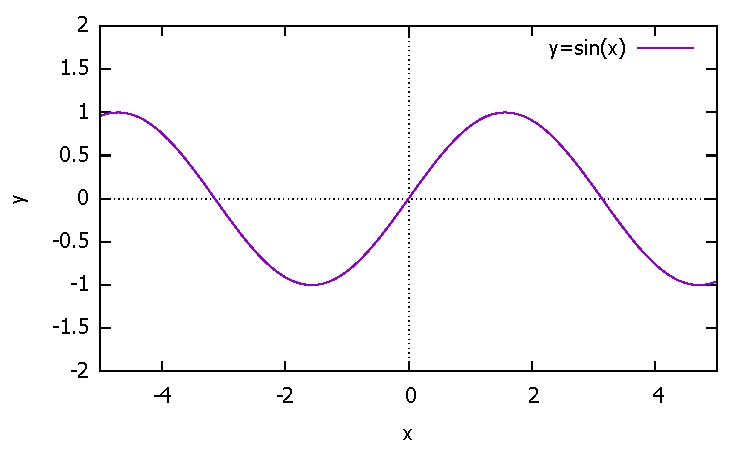
\includegraphics[width=10cm]{img/fig-sin.pdf}
%  \caption{$y=\sin x$のグラフ。gnuplotで作成した。}
%  \label{fig:sin}
%\end{figure}
%
%図\ref{fig:sin}より、sinが{\bfseries うねうね}であることがわかる。

%
%\subsection{ascmacパッケージ}
%枠で囲める。
%\begin{itembox}[l]{定義(ゼータ関数)}
%  $\Re(s) > 1$である任意の複素数$s$について、リーマンのゼータ関数$\zeta (s)$を以下のように定義する:
%  \begin{align*}
%    \zeta (s) := \sum_{n=1}^\infty \frac{1}{n^s}
%    \equiv \frac{1}{1^s} + \frac{1}{2^s} + \frac{1}{3^s} + \frac{1}{4^s} + \cdots
%  \end{align*}
%\end{itembox}

%
%\subsection{作図}
%\LaTeX と連携できるものとしては、picture環境やTi{\itshape k}ZやgnuplotやInkscapeなど色々な方法がありますが、ここではキーワードを挙げるに留めておきます。
%手描きを写真で撮ったり\footnote{明るさとコントラストをあげればそこそこキレイになる。}、パワポとかで作っても良いと思います\footnote{jpegは圧縮されて汚いので、pngか、ベクター形式のsvgとかpdfで作ると良い。}。

%
%\subsection{ソースコード}
%プログラムなどのソースコードを表示するにはlisting.styを使えばキレイに出力できますが、日本語に厳しい。そこで誰かが作ったplistings.styを代わりに使ってください。使い方はlisting.styと同じなので、そちらをキーワードにしてググってくだ
